\section{Results and Discussion}

A pair of experiments was performed to assess the evolvability of the denoising autoencoder and the bottleneck decoder genotype-phenotype maps in relation to the direct genotype-phenotype map.
A high-level overview of these experiments is provide immediately below.


First, in evolvability signature experiments the novelty and deleteriousness of mutation was assessed under these three genotype-phenotype maps.
Populations of 300 individuals were evolved using a particular map for 50 generations.
Then, the individual with the best fitness score over those 50 generations was isolated.
Mutant offspring of that individual were assessed for phenotypic novelty in relation to their parent and fitness score.
Phenotypic novelty was assessed as the euclidean distance between a parent phenotype $\vec{p}$ and a child phenotype $\vec{x}$.
Fitness was calculated according to the same criteria used during the 50 generations of evolution (described below).
Forty replicate evolutionary runs were performed for each genotype-phenotype map.
For each replicate run, 10,000 mutant offspring of the sampled champion were assessed.
The novelty and fitness scores of these mutant offspring (pooled over all 40 replicate runs) was used to generate the evolvability signatures presented in Section \ref{sec:results} \cite{tarapore2015evolvability}.

Second, experiments were performed to assess the ability of the three genotype-phenotype maps to facilitate traversal of the evolutionary search space in response to a selective pressure.
Specifically, a selective pressure for short (i.e. zero) table height was added.
Table height is calculated as the mean leg length of a table.
For each map, three replicate populations of 300 individuals were evolved for 5,000 generations.
These populations were initialized to have table height of approximately 1,000.
Response to selective pressure for short table height was assessed by tracking mean table height of the populations generation-by-generation.




\section{Results} \label{sec:results}

Assessment of evolvability signatures and observed response to selective pressure towards a global fitness peak shows that both autoencoder-derived genotype-phenotype maps enhance evolvability relative to the direct encoding.

\subsection{Evolvability Signatures}

\begin{figure*}
  \begin{subfigure}[b]{0.33\linewidth}
    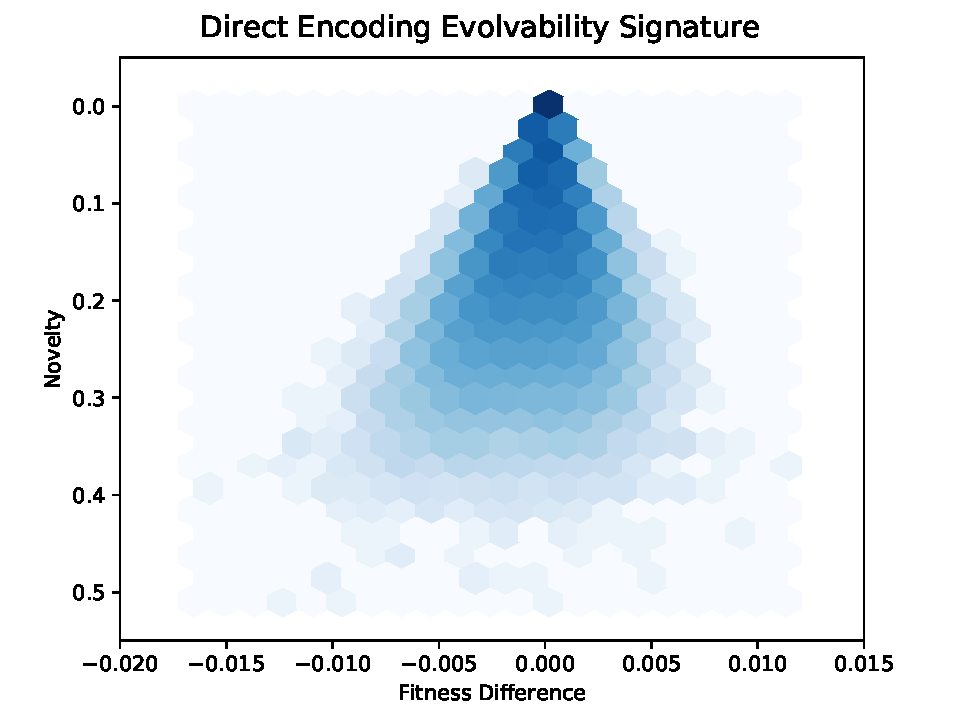
\includegraphics[width=\linewidth]{img/direct_es_unscaled}
    \subcaption{
      direct map
    }\label{fig:table_direct_es}
  \end{subfigure}
  \begin{subfigure}[b]{0.33\linewidth}
    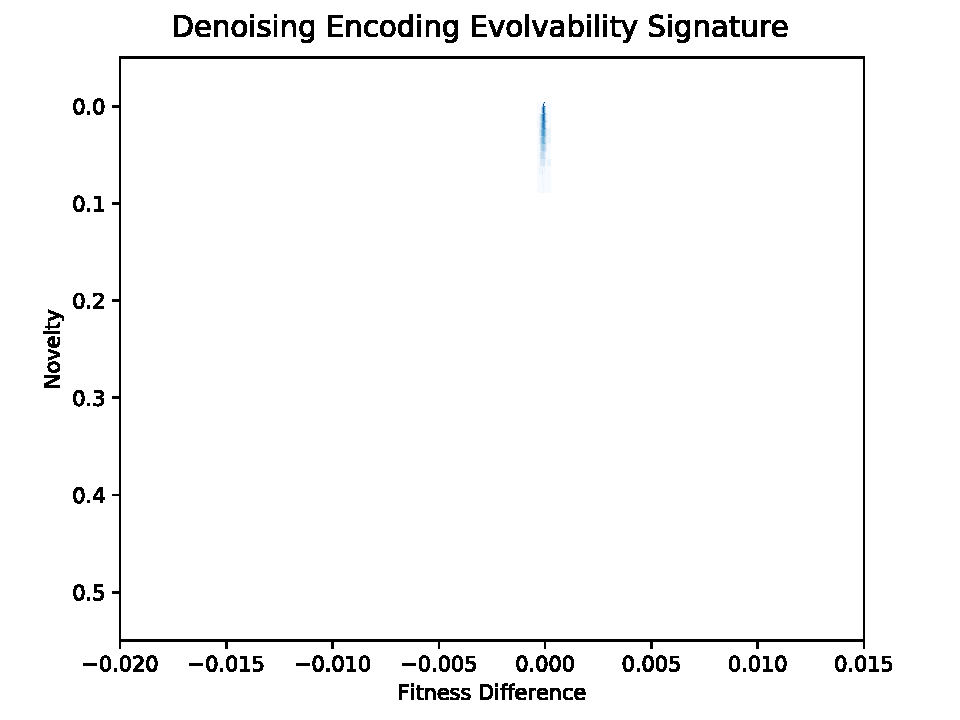
\includegraphics[width=\linewidth]{img/noise_es_unscaled}
    \subcaption{
      denoising map
    }\label{fig:table_noise_es}
  \end{subfigure}
  \begin{subfigure}[b]{0.33\linewidth}
    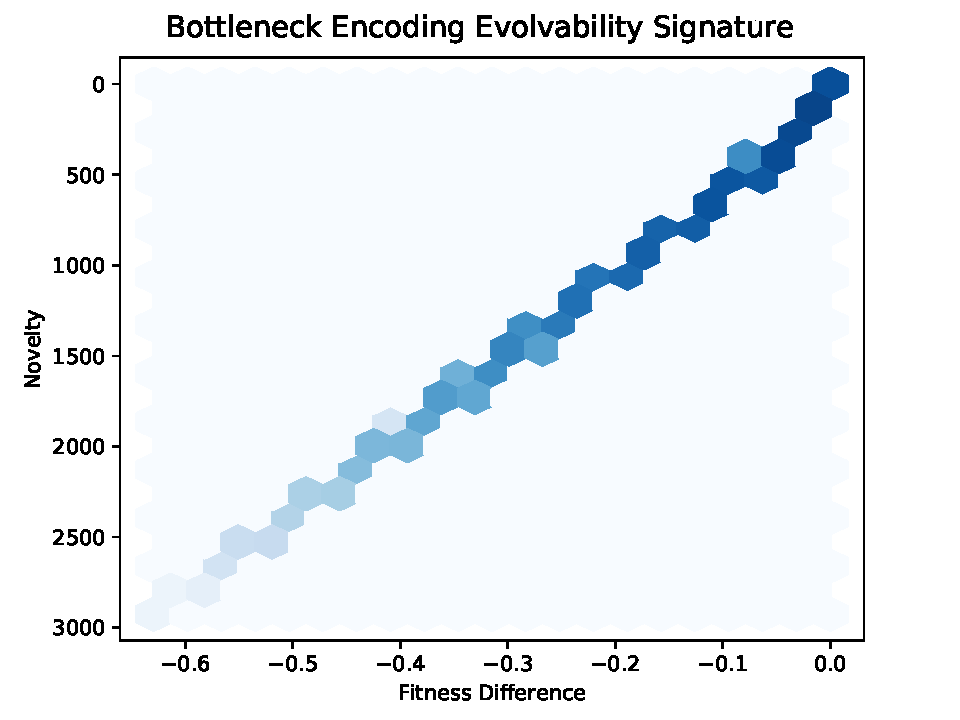
\includegraphics[width=\linewidth]{img/bottleneck_es_unscaled}
    \subcaption{
      bottleneck map
    }\label{fig:table_bottleneck_es}
  \end{subfigure}
  \caption{
    Evolvability signatures for three genotype-phenotype maps in the $n$-legged table problem domain.
    Note that subfigure \ref{fig:table_bottleneck_es} is presented with different axis scaling than subfigures \ref{fig:table_direct_es} and \ref{fig:table_noise_es}.
  }\label{fig:all_es}
\end{figure*}

\begin{figure}
        \begin{subfigure}[b]{0.33\textwidth}
                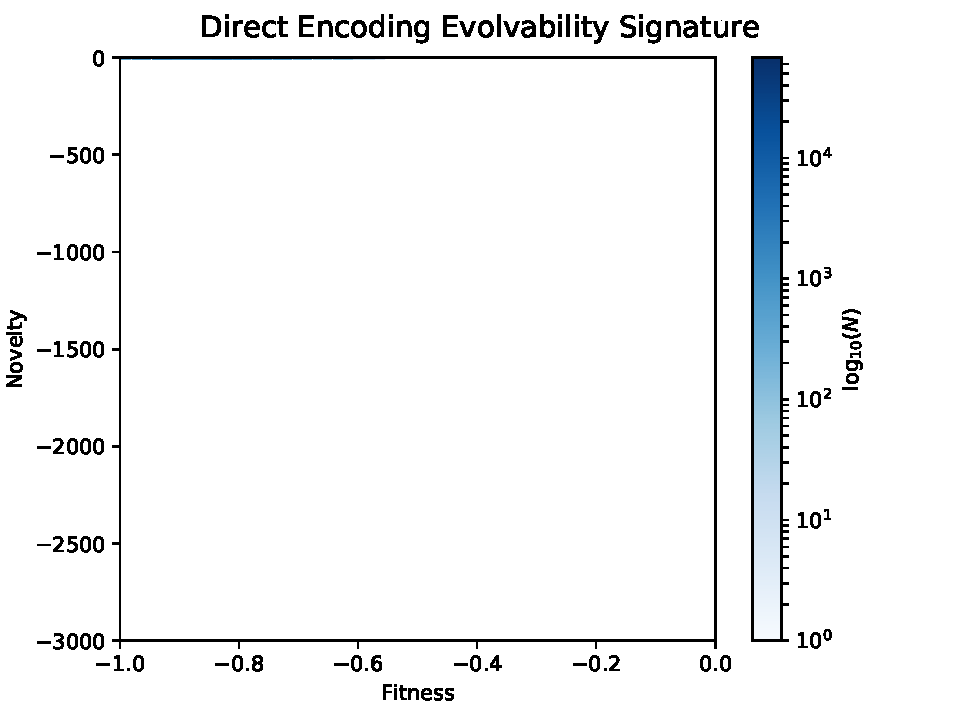
\includegraphics[width=\linewidth]{img/direct_es_scaled}
        \end{subfigure}%
        \begin{subfigure}[b]{0.33\textwidth}
                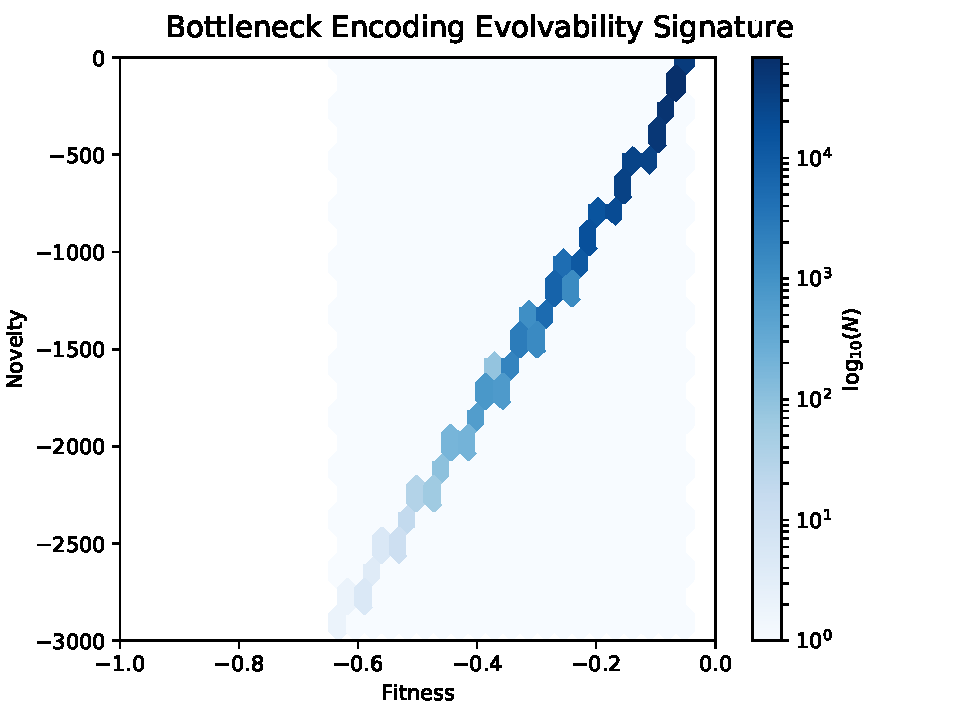
\includegraphics[width=\linewidth]{img/bottleneck_es_scaled}
        \end{subfigure}%
        \begin{subfigure}[b]{0.33\textwidth}
                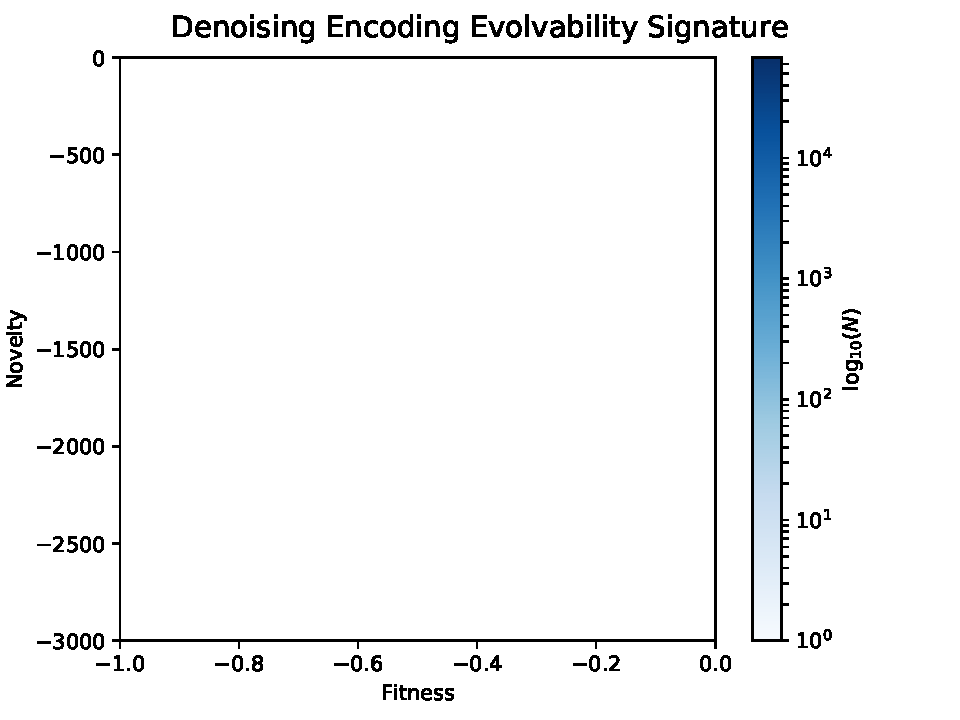
\includegraphics[width=\linewidth]{img/noise_es_scaled}
        \end{subfigure}
        \caption{Same-scale evolvability signatures for, left to right, direct bottleneck, and denoising genotype-phenotype maps.}
        \label{fig:all_es_scaled}
\end{figure}

\begin{figure}
        \begin{subfigure}[b]{0.5\textwidth}
                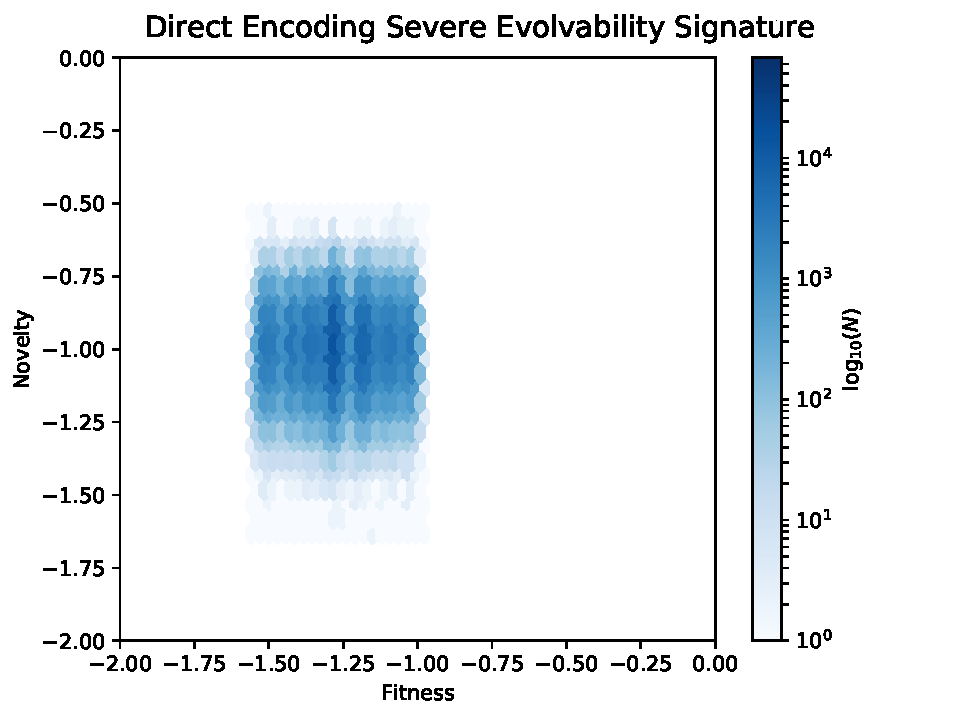
\includegraphics[width=\linewidth]{img/direct_severe_es_scaled2}
        \end{subfigure}%
        \begin{subfigure}[b]{0.5\textwidth}
                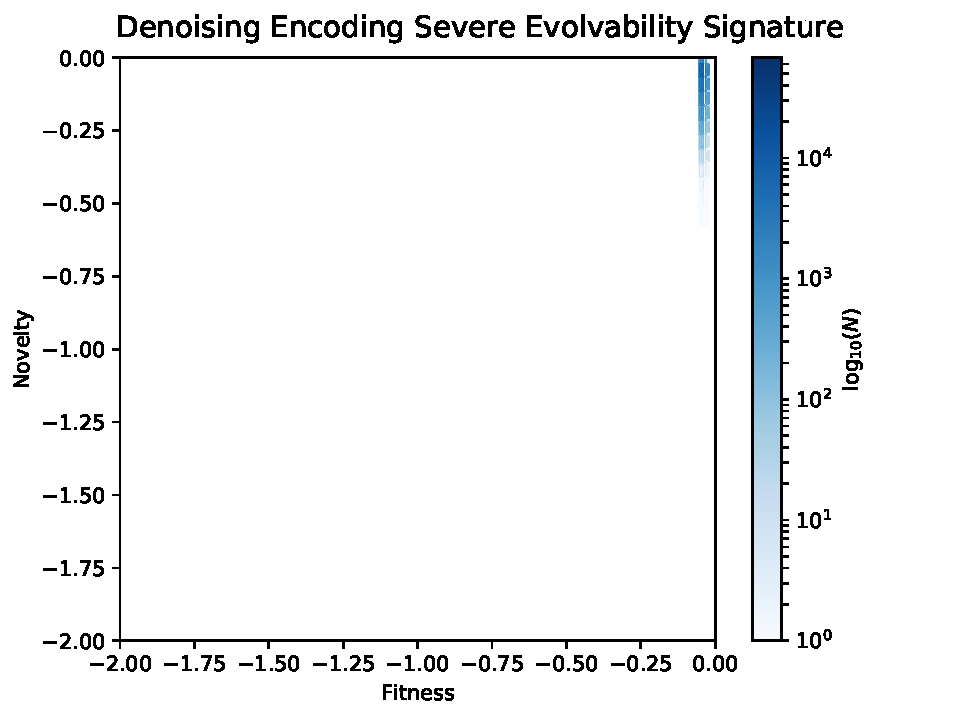
\includegraphics[width=\linewidth]{img/noise_severe_es_scaled2}
        \end{subfigure}
        \caption{Same-scale severe evolvability signatures for, left to right, direct and denoising genotype-phenotype maps.}
        \label{fig:noise_severe_compare_es}
\end{figure}



Figure \ref{fig:all_es} provides evolvability signatures for the direct, bottleneck, and denoiser genotype-phenotype maps.
These evolvability signatures are heat maps that summarize the outcomes observed under mutation for

As is expected, in all the direct and bottleneck evolvability signatures, offspring fitness tends to decrease somewhat as is expected.
Surprisingly, under the denoising mapping this is not true.
This suggests that the denoising mapping is better able to generate novelty without losing of fitness or, put another way, that mutation tends to be mildly deleterious.

It must be noted that in Figure \ref{fig:all_es}, the evolvability signature for each genotype-phenotype map are at radically different absolute scales.
Figure \ref{fig:all_es_scaled.tex} compares the evolvability signatures of the three genotype-phenotype maps at the same absolute scale.
It can clearly be seen that the bottleneck mapping can generate much more novelty per mutational step than either of the other mappings.
Note that the absolute fitness scores of nearly all offspring under the bottleneck mapping are greater than the absolute fitness of offspring under the direct mapping.
The same is true of the denoising mapping.

Because mutation under the direct and denoising mappings tend to have relatively small phenotypic effects, ``severe'' evolvability signatures were generated to better compare the evolvability of these two mappings.
These severe signatures, shown in Figure \ref{fig:noise_severe_compare_es}, are generated as before, except instead of applying a single mutation to generate mutant offspring from a parent 100 mutations were applied.
Thus, these charts reflect the novelty and fitness outcomes of larger mutational steps in the genotype space.
From this comparison, it can be seen that somewhat greater novelty tends to be generated under the direct mapping.
However, much better fitness outcomes are observed with the denoising mapping.
Again, novelty seems to be generated with little or no fitness cost.
Thus, the denoising mapping appears to produce more useful variation than the direct mapping.

\subsection{Response to Selection}

\begin{figure}
  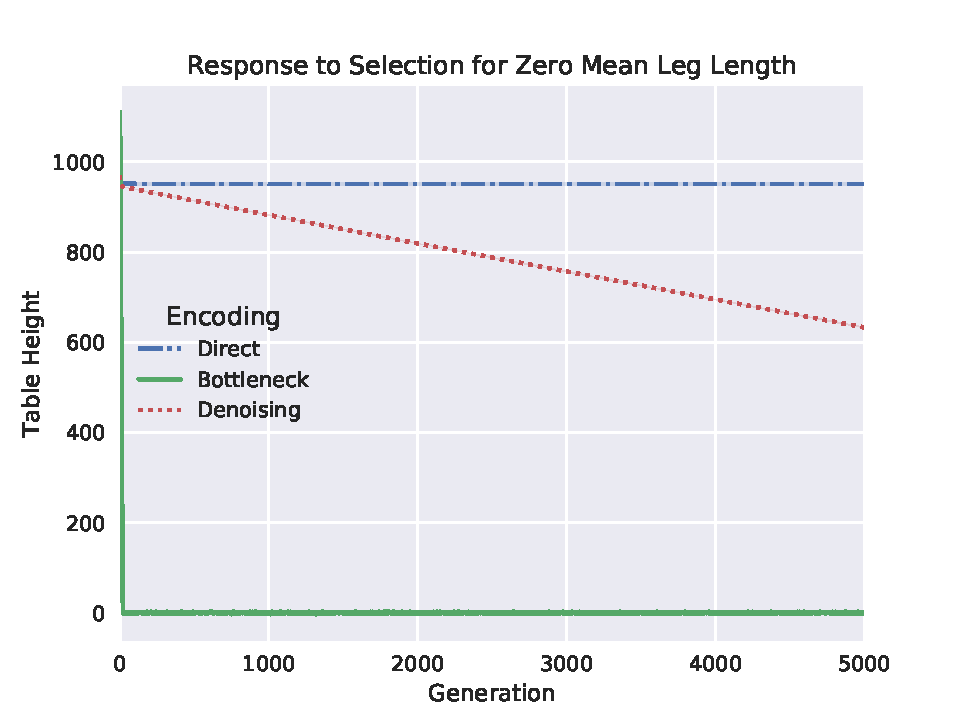
\includegraphics[width=\linewidth]{img/zero_leg_selection}
  \caption{Response to short-table selection pressure under different genotype-phenotype maps.}
  \label{fig:select_response}
\end{figure}


Figure \ref{fig:select_response} plots mean table height by generation under selection for both short table height and table stability (described in detail in Section \ref{sec:methods}).
Error bars representing standard deviation between three replicate runs, although so minuscule as not to be easily visible, are provided every 1,000 generations.

Under the direct mapping, a slight decrease in mean table height is observed for a few generations after initialization.
However, no further decrease in mean table height was observed over the course of evolutionary runs.
These runs ended with a mean table height of approximately 950.
Direct-encoded populations were trapped at local fitness peaks and unable to respond to selective pressure for short table height.

Under the bottleneck mapping, a severe decrease in mean table height is observed after initialization.
Well within 100 generations, the populations have come close to the global fitness peak --- a level table with height 0.
Populations with the bottleneck mapping were able to quickly respond to selective pressure for short table height.

Finally, under the denoising mapping, a slight drop-off in mean table height is observed after initialization.
Then, a steady decrease in table height was observed for the remainder of the evolutionary runs.
These runs ended with a mean table height of approximately 630.
Although not as quickly as under the bottleneck mapping, under the denoising mapping populations were still able to respond to selective pressure for short table height.
